\documentclass[10pt]{article}
\setlength{\parskip}{0.25\baselineskip}
\usepackage[margin=1in]{geometry} 
\usepackage{amsmath,amsthm,amssymb, graphicx, multicol, array}
\usepackage[font=small,labelfont=bf]{caption}
 

\newenvironment{problem}[2][Problem]{\begin{trivlist}
\item[\hskip \labelsep {\bfseries #1}\hskip \labelsep {\bfseries #2.}]}{\end{trivlist}}

\begin{document}
 
\title{Homework \#7}
\author{Eric Tao\\
Math 235: Homework \#7}
\maketitle
 
\section*{2.1}

\begin{problem}{4.5.17}

Show that if $f \in L^1(\mathbb{R})$ then its indefinite integral $F(x) = \int_0^x f(t)dt$ is uniformly continuous on $\mathbb{R}$.

\end{problem}
\begin{proof}[Solution]

First, we remark on the shape of $d(F(x), F(y))$. By definition of $F(x)$, $|F(x) - F(y)| = |\int_0^x f(t) dt - \int_0^y f(t) dt|$. Wlog, we can take $x > y$, as otherwise, due to the absolute value, we can just look at $|F(y) - F(x)|$. Regardless then, if $x > y > 0$, then we have that $[0,y] \cup [y,x] = [0,x], \int_0^x f = \int_0^y f + \int_y^x f$, so $d(F(x),F(y)) = \int_y^x f$. If $x > 0 > y$, we have that $[y,0] \cup [0,x] = [y,x]$, and $\int_0^x f - \int_0^y f = \int_0^x + \int_y^0 f = \int_y^x f$. And finally, if we have $0 > x > y$, we have that $[y,x] \cup [0,x] = [y,0]$, so $\int_0^x f - \int_0^y f = - \int_x^0 f + \int_y^x f + \int_x^0 f = \int_y^x f$. Regardless of case, after taking the absolute value, we can see that $|F(x) - F(y)| = |\int_y^x f| \leq \int_{[y,x]} |f|$, where we apply the fact that $|\int_E f| \leq \int_E |f|$.

Now, let $\epsilon > 0$ be given. First, by theorem 4.5.12, we have that because $f \in L^1(\mathbb{R})$, there exists a really simple function $\phi = \Sigma_{k=1}^N c_k \chi_{[a_k,b_k)}$ such that $\Vert f - \phi \Vert_1 < \epsilon/2$, and we can denote its max $c_{\max}$ out of the values that $\phi$ achieves. Now, pick $d(x,y) < \delta = \epsilon/2|c_{\max}$, and consider the interval $I =[x,y], |I| < \delta$.Then, consider a triangle inequality on $| f | = | f - \phi + \phi | \leq | f - \phi |  + | \phi |$. Since this is true everywhere, this extends to an inequality on the integrals of form:

$$ \int_I |f| \leq \int_I |f - \phi| + \int_I |\phi|$$. 

Since $| f - \phi|$ is a non-negative function, we have that $\int_I | f - \phi| \leq \int_{\mathbb{R}} |f - \phi| = \Vert f - \phi \Vert_1  < \epsilon/2$.

Then, since $|\phi|$ is bounded above by $|c_{\max}|$, we have that:

$$ \int_I |\phi| \leq \int_I |c_{\max}| = |c_{\max}| |I| < |c_{\max}| \frac{ \epsilon}{2|c_{\max}|} = \frac{\epsilon}{2}$$

Then, for any such interval, we have that $ \int_I |f|  \leq \epsilon/2 + \epsilon/2 = \epsilon$. Since this does not depend on the points $x,y$ at all, this implies uniformly continuous.

\end{proof}

\begin{problem}{4.5.22}

Show that the conclusion of the Dominated Convergence Theorem continues to hold if we replace the hypothesis $f_n \to f$ a.e with $f_n \xrightarrow[]{m} f$.
.
\end{problem}
\begin{proof}[Solution]

Let $f_{n_k}$ be any subsequence of $f_n$. In particular, this converges to $f$ in measure. Then, there exists a subsubsequence of $f_{n_k}$ that converges to $f$ pointwise a.e. Call this subsubsequence $f_{n_{k_l}}$. By the DCT then, we have that $f_{n_{k_l}} \to f$ in the $L^1$ norm becuase if for all $n$, $|f_n(x)| \leq g(x)$, then surely $|f_{n_{k_l}}| \leq g$ for all $n_{k_l}$. Then, because the choice of subsequence was arbitrary, we can always find a subsubsequence of our subsequence that converges in the $L^1$ norm. Then, by problem 1.1.22, we have that $f_n \to f$ in the $L^1$ norm, exactly the conclusion of the DCT.

Proof of 1.1.22:

Let $\{ x_n \}$ be a sequence such that for every subsequence $\{ x_{n_k} \}$, it admits a subsubsequence $\{ x_{n_{k_l}} \} \to x$, i.e. convergent to $x$. Suppose that $\{ x_n \} \not \to x$. Then, fix an $\epsilon > 0$, there exists a subsequence $\{ x_{n_m} \}$ such that $|x - x_{n_m}| > \epsilon$ for all $n_m \in \mathbb{N}$. However, by hypothesis, this subsequence admits a subsubsequence convergent to $x$, that is, we can find a subsequence $\{ x_{n_{m_i}} \}$ such that for all $n_{m_i} > M$ for some $M, |x  -  x_{n_{m_i}}| < \epsilon$, a contradiction.

Thus, if every subsequence admits a subsubsequence such that the subsubsequence converges to a value, the full sequence converges to the same value.
\end{proof}

\begin{problem}{4.5.26}

Let $E$ be a measurable subset of $\mathbb{R}^d$ such that $|E| < \infty$. Prove that $\lim_{h \to 0} |E \cap (E + h)| = |E|$.

\end{problem}

\begin{proof}[Solution]

Let $\{ n_k \}_{k=1}^\infty$ be any sequence such that $n_k \to 0$. Consider the sequence of functions $f_{n_k} = \chi_E \chi_{E + n_k}$, as well as $f = \chi_E$. We notice that this function attains $1$ on $E \cap E + n_k$ and $0$ everywhere else. We notice that $\lim_n f_{n_k} \to f$ everywhere, and $|f_{n_k}| \leq f$ everywhere. Further, $\int_E f =|E| < \infty$, thus integrable. Thus, by the DCT, we have that $\lim_k \int_E f_{n_k} = \lim_E f$. But, we have that  $\int_E f_{n_k} =  |E \cap (E + n_k)| $, and $\int_E f = |E|$. So, we have that $\lim_{k \to \infty}  |E \cap (E + n_k)| = |E|$. But, the choice of $n_k$ was arbitrary, so this works for any sequence going to $0$. Thus, we have that $\lim_{h \to 0} |E \cap (E + h)| = |E|$.

\end{proof}

\begin{problem}{4.5.27}

This problem will establish a Generalized Dominated Convergence Theorem. Let $E$ be a measurable subset of $\mathbb{R}^d$. Assume that:

(a) $f_n, g_n, f,g, \in L^1(E)$

(b) $f_n \to f$ pointwise a.e.

(c) $g_n \to g$ pointwise a.e.

(d) $|f_n| \leq g_n$ a.e

(e) $\int_E g_n \to \int_E g$.


Prove that $\int_E f_n \to \int_E f$ and $\Vert f - f_n \Vert_1 \to 0$

\end{problem}

\begin{proof}[Solution]

We proceed similarly to the proof of the DCT. We start by looking at extended real-valued functions first, as we can always just look at real/imaginary parts of a complex function. We notice that by (d), this implies that the $g_n$ must be non-negative almost everywhere. Since $g_n \to g$ pointwise, this must be true for $g$ as well. Then we have that $0 \leq \int_E g_n = \int_E |g_n| < \infty$.

Now, first, we assume $f_n \geq 0$ a.e. Then, we can use Fatou's lemma, along with (d) to see that since $f_n \leq g_n \text{ a.e.} \implies \int_E f_n \leq \int_E g_n$ for each n to see that:

$$ 0 \leq \int_E f = \int_E \liminf_n f_n \leq \liminf \int_E f_n \leq \liminf \int_E g_n  =\int_E g < \infty$$

Thus, we have that $\int_E f \leq \liminf \int_E f_n $.

We do the same with $g_n - f_n \geq 0$:

$$\int_E g - \int_E f = \int_E (g-f) = \int_E \liminf_{n \to \infty} (g_n - f_n) \leq \liminf_{n \to \infty} \int_E g_n - f_n = $$
$$\liminf_{n \to \infty} \left( \int_E g_n - \int_E f_n \right) = \liminf_{n \to \infty} \int_E g_n - \limsup_{n \to \infty} \int_E f_n = \int_E g - \limsup_{n \to \infty} \int_E f_n$$

where again, we use the convergence of $\int_E g_n \to \int_E g$ to take the $\liminf \int_E g_n \to \int_E g$.

Subtracting $\int_E g$ from both sides, and multiplying by $-1$, we get that $\int_E f \geq \limsup \int_E f_n$. So, we find that 

$$ \int_E f \leq \liminf \int_E f_n \leq \limsup \int_E f_n \leq \lim \int_E f$$

where we use the fact that $\liminf \leq \limsup$. Then, the limit exists by the squeeze theorem, and $\lim_n \int_E f_n = \int_E f$.

Now, let $f, f_n$ be any integrable functions that still satisfy (a),(b), and (d), that is, not necessarily non-negative. Consider then $|f - f_n|$. These are non-negative functions, and by the triangle inequality, we have that:

$$ |f - f_n| \leq |f| + |f_n| \leq g + g_n $$.

So, we have that: 

(b) $|f - f_n| \to 0$ pointwise a.e.

(a) $|f - f_n|$ integrable since it's nonnegative, and less or equal to $g + g_n$, a sequence of a sum of integrable functions

(c) $g + g_n \to 2g$ pointwise a.e.

(d) $|f - f_n| \leq g + g_n$ a.e.

(e) $\int_E g + g_n \to \int_E 2g$ because we already have that $\int_E g_n \to \int_E g$

Then, we have that $\lim_n \Vert f - f_n \Vert_1 = \lim_n \int_E |f - f_n| = \int_E 0 = 0$. Thus, we have that $f_n \to f$ in the $L^1$-norm, as desired.
\end{proof}

\section*{2.2}


\begin{problem}{4.6.12}

Let $Q = [0,1]^2$ and let $Q_1, Q_2,...$ be an infinite sequence of nonoverlapping squares as shown below.

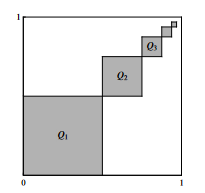
\includegraphics[width=\linewidth]{squares}
\captionof{figure}{}

Subdivide each square $Q_n$ into four equal subsquares, and let $f = 1/|Q_n|$ on the lower left and upper right subsquares of $Q_n$, and $f = -1/|Q_n|$ on the lower right and upper left subsquares. Set $f = 0$ everywhere else. Prove that:

$$ \int_0^1 (\int_0^1 f(x,y)dx)dy =  \int_0^1 (\int_0^1 f(x,y)dy)dx = 0$$

but $\iint_Q |f(x,y)| (dxdy) = \infty$. Use this to show that $\iint_Q f(x,y) (dxdy)$ is undefined.

\end{problem}
\begin{proof}[Solution]

First consider the iterated integrals, and for example, we'll look at $ \int_0^1 (\int_0^1 f(x,y)dx)dy$. In particular, we look at $\int_0^1 f(x,y)dx$. Fix any $y$ coordinate, and call it $y_0$. Regardless of the sidelength of the $Q_i$s, at a fixed $y_0$, we run horizontally through exactly one of the $Q_i$, suppose it is $Q_{n_0}$. Taking the integral along $x$ then, we notice that on one half of $Q_{n_0}$, it will equal $ 1/|Q_n|$ over an interval of length $\sqrt{Q_n}/2$ and $-1/|Q_n|$ over the same length, in some order, and 0 else. Then, the integral will equal 0 on the inside, and the integral on the outside will be over 0, so 0. This will align with the other iterated integral, as we notice slices in $x$ are the same as slices in $y$ due to the reflectional symmetry over the $y = x$ axis.

However, now consider $\iint_Q |f(x,y)| (dxdy)$. Since on any $Q_n$, $f = \pm 1/|Q_n|, |f| = 1/|Q_n|$. Then, we can say that because $|f|$ is 0 outside of the squares, and constant on them, that we can express $|f| = \Sigma_n^\infty 1/|Q_n| \chi_{Q_n}$. Then, we'd have that $\iint_Q |f(x,y)| (dxdy) = \Sigma_n^\infty \iint_{Q_n}  1/|Q_n| \chi_{Q_n} = \Sigma_n^\infty 1/|Q_n| \ast |Q_n| =  \Sigma_n^\infty 1 = \infty$, where we split the integral due to the $Q_n$ being disjoint. But if we consider $f^+$, we notice that since $f$ is positive on exactly half of each square, we have that for each $Q_n$, $\iint_{Q_n} f^+ = 1/2 \iint_{Q_n} |f|$. Then, we would have that $\iint_Q f^+ = \Sigma_n^\infty \iint_{Q_n} f^+ = \Sigma_n^\infty 1/2 \iint_{Q_n} |f| = \Sigma_n^\infty 1/2 = \infty$. However, this argument works for $f^-$ as well, since half of each square takes on $-1/|Q_n|$. Then, we have that $\iint_{Q} f^+ = \infty = \iint_{Q} f^-$, so the integral is undefined.

\end{proof}

\begin{problem}{4.6.20}
Given $f \in L^1[0,1]$ define

$$g(x) = \int_x^1 \frac{f(t)}{t} dt, 0 < x \leq 1$$

Show that $g$ is defined a.e. on $[0,1], g \in L^1[0,1]$ and $\int_0^1 g(x)dx = \int_0^1 f(x)dx$.
\end{problem}
\begin{proof}[Solution]

First of all, we see that $g$ is defined a.e. on $[0,1]$. Let $\delta > 0$ be given. Then, consider $g(\delta) = \int_\delta^1 \frac{f(t)}{t} dt$. In particular, we have that $|\frac{f(t)}{t}| \leq |\frac{f(t)}{\delta}|$ for all $t \in [\delta,1]$. Then, we have that, $\int_{[\delta,1]} | \frac{f(t)}{t}| \leq \int_{[\delta,1]}  |\frac{f(t)}{\delta}|= 1/\delta \int_{ [\delta,1]} |f(t)| \leq 1/\delta \Vert f \Vert_1$. Since, in particular, we have that $f^+, f^- \leq |f|$ everywhere by definition, we have that both integrals are bounded on $[\delta,1]$. Since the choice of $\delta > 0$ was arbitrary, this works for any such $\delta$ and may only fail at $x =0$, a set of measure 0. So we are defined a.e.

Now, since $f \in L^1$, $f$ must be finite almost everywhere, since otherwise there's a set of postive measure where $f$ is infinite, thus $\int |f| = \infty$, a contradiction. Further, the function $g(t) = t$ is only $0$ at $t = 0$, a set of measure 0 in $[0,1]$. Thus, by lemma 3.2.4, we have that $f(t)/g(t) = f(t)/t$ is measurable on $t \in [0,1]$.

Consider the lift of this function into $f: E \to \overline{F}$ where $E$ is the lower-right half-triangle on the unit square in the $t$-$x$ plane. That is, the triangle given by $x = 0, x  = 1, x = t$. Then, we will apply Tonelli's theorem here, by extending this function to $h(x,t)$ such that $h(x,t) = 0$ when $0 < t < x$, and $f(t)/t$ otherwise, which is measurable because it looks like $\chi_E f(t)/t$, the product of measurable functions. Firstly, by (d), we have that $g(x) = \int_{[0,1]}  h^x(t) dt = \int_{[x,1]} f(t)/t dt$ is measurable, where we've used the fact that $h = 0$ on $t \in [0,x]$ for each slice at $x$. Further, we see that:

$$\iint_{[0,1]\times [0,1]} h(x,t) (dxdt) = \int_{[0,1]} \left( \int_{[0,1]} h(x,t) dx \right)dt =\int_{[0,1]} \left( \int_{[0,1]} h(x,t) dt \right)dx $$

In particular, we notice:

$$ \int_{[0,1]} \left( \int_{[0,1]} h(x,t) dt \right)dx = \int_{[0,1]} \left( \int_{[x,1]} \frac{f(t)}{t} dt \right) dx =  \int_{[0,1]} g(x) dx  $$

and

$$  \int_{[0,1]} \left( \int_{[0,1]} h(x,t) dx \right)dt = \int_{[0,1]} \left( \int_{[0,t]}  \frac{f(t)}{t}  dx \right)dt = $$

$$ \int_{[0,1]} \left( \frac{f(t)}{t} \ast x \Big|_0^t \right)dt = \int_{[0,1]} f(t) dt$$

Then, we have that:

$$\int_{[0,1]} g(x) dx = \int_{[0,1]} \left( \int_{[x,1]} \frac{f(t)}{t} dt \right) dx =  \int_{[0,1]} f(t) dt$$

Lastly, by corollary 4.6.9 on $h$, we have that:

$$\iint_{[0,1]\times [0,1]} |h(x,t)| (dxdt) = \int_{[0,1]} \left( \int_{[0,1]} |h(x,t)| dx \right)dt =\int_{[0,1]} \left( \int_{[0,1]} |h(x,t)| dt \right)dx $$

and then we have that:

$$\int_{[0,1]} |g(x)| dx = \int_{[0,1]} \left| \int_{[x,1]} \frac{f(t)}{t} dt \right| dx \leq  \int_{[0,1]} \left( \int_{[x,1]} \left|\frac{f(t)}{t}\right| dt\right) dx = $$

$$ \int_{[0,1]} \left( \int_{[0,1]} \left|h(t) \right| dt\right) dx =  \int_{[0,1]} \left( \int_{[0,1]} |h(x,t)| dx \right)dt = \int_{[0,1]} \left( \int_{[0,t]} \left| \frac{f(t)}{t} \right|  dx \right)dt =$$

$$  \int_{[0,1]} \left( \left| \frac{f(t)}{t}\right| \ast x \Big|_0^t \right)dt = \int_{[0,1]} \left|f(t) \right| dt < \infty $$

where we notice we use the fact that $x,y \geq 0$ to conclude that $\left| f(t)/t\right| \ast x \Big|_0^t = \left| f(t)/t \right| t = \left| f(t) \right| $. Thus, $g \in L^1([0,1])$.

\end{proof}

 

\end{document}